% This is samplepaper.tex, a sample chapter demonstrating the
% LLNCS macro package for Springer Computer Science proceedings;
% Version 2.20 of 2017/10/04
%
\documentclass[runningheads]{llncs}
%\usepackage{amsthm}
\usepackage{graphicx}
% Used for displaying a sample figure. If possible, figure files should
% be included in EPS format.
%
% If you use the hyperref package, please uncomment the following line
% to display URLs in blue roman font according to Springer's eBook style:
% \renewcommand\UrlFont{\color{blue}\rmfamily}

\begin{document}
%
\title{Streaming Massive Electric Power Data Analysis Based on Spark Streaming\thanks{Supported by organization x.}}
%
%\titlerunning{Abbreviated paper title}
% If the paper title is too long for the running head, you can set
% an abbreviated paper title here
%
\author{First Author\inst{1}\orcidID{0000-1111-2222-3333} \and
Second Author\inst{2,3}\orcidID{1111-2222-3333-4444} \and
Third Author\inst{3}\orcidID{2222--3333-4444-5555}}
%
\authorrunning{F. Author et al.}
% First names are abbreviated in the running head.
% If there are more than two authors, 'et al.' is used.
%
\institute{Princeton University, Princeton NJ 08544, USA \and
Springer Heidelberg, Tiergartenstr. 17, 69121 Heidelberg, Germany
\email{lncs@springer.com}\\
\url{http://www.springer.com/gp/computer-science/lncs} \and
ABC Institute, Rupert-Karls-University Heidelberg, Heidelberg, Germany\\
\email{\{abc,lncs\}@uni-heidelberg.de}}
%
\maketitle              % typeset the header of the contribution
%
\begin{abstract}
Electric power user classification is one of the most important methods to realize the optimal allocation of power resources. Through the analysis of users'needs, behavior and habits, Countries and enterprises can offer different incentives for different users. In this way, people are more willing to use green and clean Electric power resources. In the analysis of user clustering, there is a need for real-time processing of massive and high-speed data. In this paper we propose a novel distributed user data stream clustering method based on Spark streaming, improved clusStream algorithm and improved K-means algorithm named "DStreamEPK". In the final experimental evaluation, we first tested the clustering effectiveness of DStreamEPK on UCI datasets, the results show that the proposed DStreamEPK is better than the traditional K-means clustering algorithm. At the same time, it is found that DStreamEPK can cluster user's electricity data quickly and efficiently through testing on user's real data sets.

\keywords{Spark Streaming  \and ClusStream \and K-means \and Electric Power.}
\end{abstract}
%
%
%
\section{Introduction}

 In recent years, people all over the world are increasingly demanding to protect the environment and achieve sustainable development. In this context, how to make electricity consumption behavior intelligent has become a very important research topic. A great deal of basic electricity consumption data have been accumulated\cite{muchData}. These data are huge and high Frequency. At the same time, the user's electricity data is constantly generated. The newly generated electricity data can better reflect the user's electricity characteristics. Distributed clustering of the user's electricity data can provide different incentives for different users. This way can help grid companies to understand the user's consumption habits and provide personalized and differentiated services for users. Furthermore, it helps companies to further expand the depth and bread th of their services, and provides data support for the formulation of future power demand response policies. At the same time, the company will timely feedback the residential power consumption data and residential power consumption to users, so that users can understand their own electricity consumption information and contribute to low-carbon environmental protection.
 
 Cluster analysis is a classical method in the field of data mining. Wang\cite{wang} proposed a short-term load forecasting method for power system. Zhao\cite{zhao} proposed an improved K-means based clustering method for power load curve..
 
 In the meantime, many stream clustering methods have been proposed. Birch\cite{birch} algorithm is a hierarchical clustering algorithm proposed by T. Zhang et al in 1996. C.C. Aggarwal et al proposed ClusStream\cite{clusStream}, a classical two-tier data stream processing framework in 2003. T Rakthanmanon et al proposed E-Stream\cite{E-stream} clustering algorithm in 2007 to improve clusStream algorithm's poor clustering performance for high-bit data. I.Assent et al\cite{clusTree} proposed Clustree algorithm in 2011 to cluster data points with arbitrary shape distribution effectively. R. Marcel et al proposed StreamKM++ algorithm\cite{streamKM} in 2012.
 
 There exists a lot of clustering algorithms and Data Stream Clustering Algorithms, such as k-means\cite{kmeans} algorithm, improved version algorithm based on k-means, ClusStream,  StreamKM++ algorithm et. However, these algorithms can not be directly and efficiently applied to distributed storage and computing environments. How to integrate these algorithms into the current mainstream big data processing frameworks such as Hadoop and spark is a very worthwhile problem.
 
 However, there are few research results on data flow and distributed computing, which are still in the initial stage of exploration. In this paper, the traditional stream clustering algorithm and distributed stream processing platform are introduced firstly, and then the problems of current stream clustering algorithm are analyzed. Based on the original stream clustering algorithm, a stream clustering algorithm DStreamEPK based on SparkStreaming is proposed. DStreamEPK uses a typical two-tier clustering method to maintain the outline information of data stream in online part using X* tree; canopy is used to solve the initial K value selection problem of K-means algorithm in offline part, and an efficient distributed parallel k-means algorithm is designed to cluster power data offline.
 
 Our major contributions can be summarized as follows:
   \begin{enumerate}
     \item  A parallel k-means algorithm based on spark is designed.
     \item  Using canopy algorithm to solve k-value selection problem of K-means algorithm.
     \item  A clustering method based on spark streaming for user power data is proposed.
     \item  new stream clustering algorithm DStreamEPK is proposed.
   \end{enumerate}
 

\section{Preliminary}
\subsection{Spark Streaming}
Spark is a research product created by APMLab Laboratory at the University of California, Berkeley. It was officially open source in 2010, became an Apache Foundation project in 2013, and became the top project of the Apache Foundation in 2014.

Spark\cite{spark} mainly solves the problem of slow computation in hadoop, which is caused by repeated read and write disks.

Resilient Distribute Datasets (RDD) is the core of Spark and the key to Spark's fault recovery and data dependence.RDD model uses Lineage mechanism to solve the dependence between data, and ensures good fault tolerance. It can store intermediate results in memory and minimize disk reading and writing of data, which greatly improves the computing speed. Especially in iterative computing, the computing speed is increased by an order of magnitude.

Data does not exist in the original form in RDD, but is included in RDD in the form of the specific location of the data. New RDD is obtained through different transformations in RDD, and the real calculation is not performed until the action is executed to get the final desired result.Spark Streaming is used for real-time computing in Spark ecosystem

The essence of Spark Streaming stream processing is to merge data in a short period of time and then do micro batch processing instead of real-time processing each data separately. This is also the biggest difference from other stream processing systems, so it is not real-time processing, but microbatch processing with lower latency.
\subsection{Stream Clustering Algorithm}
C.C. Aggarwal et al. first proposed a two-layer flow clustering framework in clusStream algorithm, which regards the process of data stream clustering as a process of change, instead of computing and preserving all data with the same granularity. The algorithm can respond to users'queries and clustering requests in time, and return clustering results with different granularity.

For the first time, the algorithm divides the flow clustering process into two parts: offline clustering and online clustering. In the micro-clustering stage, micro-clusters are used to represent the clustering information in the original data. Because micro-clusters are additive, the updating of data is incremental. In the macro-clustering stage, the off-line algorithm can get the final results by clustering all the micro-clusters generated in the online stage. The algorithm introduces a pyramidal inclined time window to deal with the importance of time in different time periods. That is to say, the closer the data is to the current time, the more important it is. The clusStream algorithm uses finer granularity to save new data points in time dimension and coarser granularity to save old data points. The final data snapshot is similar to the inverted pyramid shape, as shown in the figure.

CluStream algorithm uses the clustering feature vector (CF) of BIRCH algorithm to store the outline information of data stream. CF, which first appeared in BIRCH algorithm, is a triple feature

Vector <n, LS, SS>, n is the number of data points, LS is the linear sum of n points, SS is the square sum of n points. LS and SS are vectors of the same dimension as the original data points. Because CF is additive, updates to micro clusters can be obtained by vector operations. For example, when a new data point is added to a micro-cluster, the general information of the micro-cluster can be updated by adding vectors.

In CluStream algorithm, besides time stamp T, CF of micro-cluster also maintains several other time labels - LST is the sum of time stamps, SST is the sum of time stamps. CluStream determines whether to create a new cluster or merge it into an existing one by determining the distance between the data point and its nearest cluster and the distance threshold. In order to maintain the relative stability of the number of micro-clusters, when a new micro-cluster is generated, two micro-clusters are selected from the existing micro-cluster set to merge or discard an older micro-cluster. In this way, the algorithm can keep the newer data in the micro-cluster and reduce the memory consumption. Although the algorithm has good running efficiency and better clustering accuracy, because the Euclidean distance is used to evaluate the similarity, the algorithm can only cluster data streams with spherical distribution. For data streams with other types of distribution, the algorithm can not cluster effectively, and the algorithm can not deal with outliers well.
\subsection{K-means Canopy and R Tree}
\subsubsection{K-means}
K-means is a partition-based clustering algorithm, which is simple and efficient.

Because of its strong expansibility, it has been widely used in various fields. K-means algorithm usually uses Euclidean distance between two samples as a measure of similarity.

The calculating steps of K-means algorithm are as follows: firstly, K initial clustering centers are selected artificially in DataSet, then Euclidean distances from the remaining sample data to the initial center are calculated, then each sample is classified into the corresponding cluster centers according to the principle of minimum distance, and then the average distances of all samples of each class are calculated and updated to the new cluster centers of the class. Until the sum of squares of errors function is stable at the minimum value.
\subsubsection{Canopy}
Although Canopy algorithm\cite{Canopy} does not need to set the number of clusters K, it needs to set the distance range Db and Ds, in which Db refers to the maximum distance threshold and Ds refers to the minimum distance threshold. The relationship between them is Db > Ds. The number of canopy subsets in clustering results and their data points can be affected by the setting of distance threshold. However, if the Db is too large, many points will belong to multiple Canopy at the same time, which may eventually lead to a smaller difference between the central points of each cluster, and the difference between the clusters is not obvious. If Ds is too large, it may lead to too few clusters, but if Ds is too small, it will lead to too many clusters and greatly increase the clustering time. So we must set the values of Db and Ds reasonably.

The data set R is read into memory, and then the distance threshold parameters Db and Ds are set.

A data point D is randomly selected from R and the distance from D to all canopy subsets is calculated. If there is no canopy subset at the beginning, we need to treat data point D as a new canopy list, and at the same time remove d from R. If the distance between data D and the center of a canopy is less than or equal to Db, then D is written to the canopy, but the data is not deleted from R.

If the distance between the data point D and the center of a canopy is not greater than Ds, D is written to the canopy and the node is deleted from R.

Repeat step 2, 3 until R becomes an empty data set.
\subsubsection{R Tree}
R-tree\cite{RTree} is a balanced tree used to store high-dimensional data. It solves the search problem in high-dimensional space very well. R-tree extends the idea of B-tree to multi-dimensional space, uses the idea of B-tree partitioning space, and uses the method of merging and decomposing nodes when adding and deleting operations to ensure the balance of the tree.

R-tree is an extension of B-tree in high-dimensional space and a balanced tree. The leaf nodes of each R tree contain multiple pointers to different data, which can be stored on hard disk or in memory. According to the data structure of R-tree, when we need a high-dimensional spatial query, we only need to traverse the pointers contained in a few leaf nodes to see whether the data pointed by these pointers meet the requirements. This way we can get the answer without traversing all the data, and the efficiency is greatly improved.
\section{Architecture of Analysis Model}
\begin{figure}[t]
	\centering
	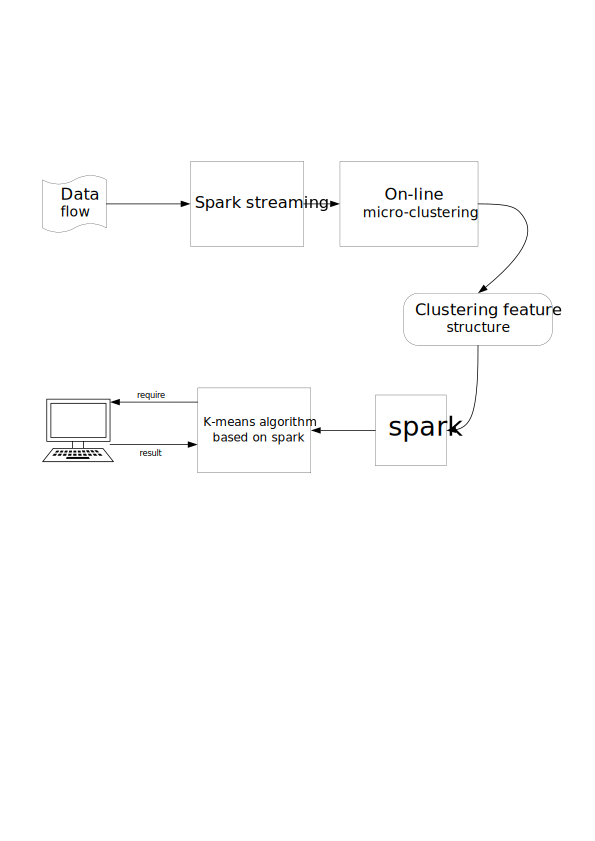
\includegraphics[height=4cm,width=9cm]{archi.jpg}
	\caption{Architecture} \label{archi}
\end{figure}%
ClustesStream algorithm points out several problems that need to be solved when designing the framework of stream clustering algorithm. These problems can be summarized as follows:
\begin{enumerate}
	\item  How to Store Data Summary Information Quickly and Efficiently in Continuous Data Stream? 
	\item  At waht moments in time should the summary information be stored away on disk?
	\item  How can the periodic summary statistics be used to provide clustering and evolution insights over user-specified time horizons?
\end{enumerate}
Referring to the algorithm framework model proposed by clusStream algorithm, we propose a framework used in DStreamEPK algorithm.

\begin{theorem}
	data frame D consists of a set of multi-dimensional records X1,X2,X3 ... arriving at timestamps T1,T2,Tk...Each Xi is a multi-dimensional record containing d dimensions.
\end{theorem}
\begin{theorem}
	We optimize mirco-cluster based on clusStream algorithm. A micro-cluster for a set of d-dimensional points Xi1...Xin with timestamps Ti1....Tin is defined as the (2*d+3) tuple (CF2x,CF1x,n,tl,id), wherein CF2x and CF1x ech correspond to a vector of d entries. The definition of each of these entries is as follows:
	\begin{itemize}
		\item There are d elements in CF2x, which is the sum of squares for each dimension of data.
		\item For each dimension, the sum of the data values is maintained in CF1x.therefore,CF1x includes d values.
		\item n represents the number of elements in a microcluster. 
		\item tl is the last update time of data in micro-cluster.
		\item id is the only symbol of micro-cluster.
	\end{itemize}
\end{theorem}
\section{On-line Streaming Clustering Algorithm}
R* tree is mainly used to perform similarity search in multidimensional data. SS tree is an improved index tree based on R* tree. The original R* tree uses the form of hypercube to partition the multidimensional space, which results in a large number of overlapping nodes in the tree index. However, SS tree uses hypersphere method to divide space. SS tree does not need any additional data besides the central point and radius of subspace, so it can save space and improve the speed of search.

The algorithm based on SS-Tree is executed as follows:
\begin{enumerate}
	\item Initialization of SS tree structure
	\item Pre-clustering the received data to generate several micro-clusters
	\item When the new data point X arrives, according to whether the distance from X to the center of each micro-cluster is greater than the RMS deviation (root mean square error) of the micro-cluster, and greater than the new micro-cluster with an independent ID for the q-point, otherwise it will be added to the nearest existing micro-cluster (using the additive property of the eigenvector group). 
	\item Once a new micro-cluster is established, it is necessary to delete an original micro-cluster. In theory, it is usually determined to delete the micro-cluster according to the recent time stamp formed by the M points that have recently arrived at each micro-cluster. In practice, the mean and standard deviation of arrival time of each data point can be obtained according to the time statistics in the micro-cluster, because the default micro-cluster satisfies the normal distribution. So extracting the time information relevance time of m/(2*n) is compared with the preset threshold delta. If the minimum relevance time is less than delta, the corresponding micro-cluster can be deleted.
	\item If all relevance time values are larger than delta, two nearest micro-clusers need to be merged, and the corresponding ID is formed as an idlist.
\end{enumerate}

\subsection{Updating of Micro-Clusters}
Experience shows that the importance of data with timestamps is different, and the latest data has a greater impact on users. That is to say, data flow information has timeliness. When a part of the data exists for more than a certain period of time, it is likely that this part of the data will be de-valued. ClsStream algorithm uses pyramid time window to store micro-clusters in different time periods. In our research, we use a simpler time-decay technique to update and delete micro-clusters periodically. Time attenuation technology can make data of different time show different importance according to the set function. Setting up a process in the algorithm and updating and deleting all data at a fixed time interval can reduce the impact of historical data in this way:

The time weighting function is as follows:

In the above formula, A is the attenuation factor. The value of a reflects the role of historical data in clustering. The larger the value, the smaller the impact of historical data on the algorithm.

The time decay function of micro-clusters is calculated as follows:

\section{Off-line Streaming Clustering Algorithm}
\subsection{Preprocessing of Electricity Data}
In order to improve the efficiency of the algorithm in massive residential power data mining Rate, data need to be preprocessed, as shown in Figure 1
\subsubsection{Data filtering}
In the original residential electricity data, there may be a user's electricity information data at a certain time is repeatedly recorded, or is divided into multiple electricity information for recording. For the duplicate records, the method of direct filtering and deletion is adopted. For the latter, the user number can be extracted, and the electricity information can be superimposed and merged into a single data record. In addition, there may be some missing values in a user's data. In this case, a threshold of the number of missing values can be set beforehand. When the threshold is exceeded, the record can be deleted directly. On the contrary, only the missing values can be filtered out.
\subsubsection{Data filling}
The method to deal with the missing values is to select the average value of the two adjacent load values of the missing values as the corresponding filling values. If the neighborhood value is also empty, the next non-empty load value is found forward or backward. If there is no non-empty load value, it is filled with zero value.
\subsubsection{Normalization of features}
In the original data, after extracting the relevant user features, different eigenvalues may have different ranges. The influence of larger eigenvalues on the global matrix is greater than that of smaller ones, which weakens the role of smaller features. Therefore, it is necessary to normalize the features. In this paper, the interval normalization method is used for eigenvalue matrix X = X1 x2.. The maximum Max (xi) and minimum min (xi) of eigenvalues in the eigenvalue matrix are calculated. According to the formula (8), the eigenvalue fields are normalized to intervals [0, 1], and a set of normalized matrices V = V1 V2 are obtained. VP]
\subsection{K-Means clustering algorithm combined with Canopy}
When the number of nodes in a distributed cluster is not limited, the performance of the traditional clustering algorithm can be improved with the increase of computing nodes after it is parallelized in Park Streaming. However, when the machine is insufficient and the operation efficiency of the algorithm can not meet the needs of the application, it is also a good solution to optimize the design idea and execution logic of the algorithm itself.

In this paper, the optimization of stream clustering algorithm is mainly embodied in the selection of initial centers of K-Means clustering algorithm, the setting of K value of cluster number and the execution method of K-means algorithm on Spark cluster.

Firstly, this paper chooses Canopy rough clustering algorithm to realize the internal optimization of stream clustering algorithm. The clustering results of Canopy algorithm provide the initial clustering centers and K values for K-Means, which can effectively avoid the randomness of K-Means calculation results and reduce the running time, thus improving the processing performance of K-Means for large-scale data.

By using map(), combine() and reduce() three functions, the spark cluster is implemented efficiently.

Canopy algorithm does not need to specify the number of clusters manually. It can cluster actively according to its own iteration. It only needs to set the threshold Db and Ds in the clustering process, where Db > Ds. Therefore, Canopy rough clustering algorithm and K-Means algorithm can be combined, and the output of Canopy algorithm can be used as the input of K-Means. In this way, the subjectivity of K selection in K-Means and the randomness of initial cluster center selection can be avoided to a certain extent, so that the efficiency and accuracy of clustering can be improved by reducing the number of iterations in K-Means clustering algorithm. Based on the above analysis, the implementation steps of K-Means optimization algorithm based on Canopy are as follows:

Step 1: After data set R is preprocessed, a list of data R'is written to memory, and appropriate distance thresholds are selected: Db, Ds (Db > Ds).

Step 2: According to the Canopy method, all data in R'is divided into several Canopy.

Step 3: Use the number of Canopy generated in Step 2 as the K value of the K-means algorithm.

Step 4: Execute the K-means algorithm.

\subsection{prallel K-means on Spark}
\subsubsection{map}
Firstly, the pre-processed data set R'is read into memory and stored in the form of < key, value > in which key is the offset of the current sample relative to the starting point of the input data file, and value is a string of coordinate values of the current sample. Firstly, the value of each dimension of the current sample is resolved from value; then the distance between the current sample and K centers is calculated to find the subscript of the nearest cluster; finally, <key', value'> where key'is the subscript of the nearest cluster and value' is the string of coordinates of the current sample. The pseudocode of the function is:

In order to reduce the amount of data and communication cost in the iteration process, after Map operation, we design a Combine operation, which merges the output data after each Map function is processed locally. Because the data output after each Map operation is always stored in the local node, each Combine operation is executed locally, and the communication cost is very small.
\subsubsection{combine}
In the pair of key, Value input by Combine function, key is the subscript of cluster, and V is a string list of coordinate values of each sample assigned to cluster with subscript key. Firstly, the coordinate values of each sample are sequentially resolved from the list of strings, and the coordinate values corresponding to each dimension are added up separately. At the same time, the chain is recorded.

The total number of samples in the table. The output key', value 'is the subscript of the cluster to the middle key value is a string, which includes two parts of information: the sum and composition of the total number of samples and the coordinate values of each dimension. The function pseudocode is:

\subsubsection{Reduce}
In Reduce function input key, V key is the subscript of cluster, V is the intermediate result of transmission from each Combine function. In Reduce function, the number of samples processed from each Combine and the cumulative values of coordinates of the corresponding nodes in each dimension are firstly analyzed, and then the corresponding cumulative values of each dimension are added respectively, and then divided by the total number of samples, the new coordinates of the central points are obtained. The function pseudocode is:

According to the output of Reduce, the new center coordinates are obtained and updated. To the file on HDFS, and then the next iteration, until the algorithm converges.

\section{Experiments and Evaluations}
Based on the spark platform and the improved K-means algorithm, we have completed the following experiments. 

\subsection{Clustering validity}
In order to verify the effectiveness of the improved K-means clustering algorithm, we selected some data sets provided by UCI website, and compared the traditional K-means algorithm with the improved algorithm in this paper. The clustering results were measured by AdjustRand Index and clustering accuracy. 
\begin{figure}
	\begin{minipage}[t]{0.5\linewidth}
		\includegraphics[height=5cm,width=6cm]{k_meansResult.png}
		\caption{cluster result} \label{k_meansResult}
	\end{minipage}%
	\begin{minipage}[t]{0.5\linewidth}
		\includegraphics[height=5cm,width=6cm]{accuracy.png}
		\caption{Accuracy} \label{accuracy}
	\end{minipage}
\end{figure}
It is easy to draw the following conclusions from Figure 1 and Figure 2. Compared with the traditional K-means algorithm, the K-means algorithm combined with canopy has better clustering effect and higher accuracy. Therefore, it is very meaningful to use the improved k-means clustering algorithm in the offline part of DStreamEPK algorithm. 


\subsection{Stream Clustering Verification }
\begin{figure}
	\begin{minipage}[t]{0.5\linewidth}
		\includegraphics[height=5cm,width=6cm]{SSE.png}
		\caption{SSE} \label{SSE}
	\end{minipage}%
	\begin{minipage}[t]{0.5\linewidth}
		\includegraphics[height=5cm,width=6cm]{time.png}
		\caption{TIME COST} \label{time}
	\end{minipage}
\end{figure}
Compared with DStream EPK algorithm, CluStream algorithm runs shorter time on data set, because CluStream's online clustering and offline clustering algorithms are implemented by simple K-Means, and it controls the number of iterations. The proposed DStreamEPK algorithm needs to run canopy algorithm once in the offline phase, so it will consume more time. Overall, however, the time consumed is not too much. It is worthwhile to sacrifice part of the time for higher accuracy.


\section{Conclusions}
In this paper, the analysis of residential power consumption data is studied on the basis of a large number of user power consumption data.            
A spark streaming processing and improved K-means algorithm based user power data analysis method is proposed. 
It includes the following aspects:            

1) There are initial clustering centers and optimal K-means clustering algorithm in traditional K-means clustering algorithm. It is difficult to determine the value. In this paper, canopy algorithm is used to determine K value, which improves the clustering accuracy.            

2) An improved K-means algorithm based on spark Streaming is proposed. According to the analysis method. On-line phase can quickly collect micro-cluster information and statistical summary information. In the offline stage, the characteristics of peak-time power consumption rate, load rate, valley load coefficient and flat-section power consumption percentage of each user are extracted by pre-processing of user's power consumption data, and the data vector dimension is established. Then, the improved K-means algorithm is used to cluster the data, and the parallel algorithm is realized on the basis of spark. The user's electricity consumption behavior is analyzed and the characteristics of each type of user are extracted. The experimental results show that the proposed method is stable, efficient and reliable. A massive algorithm based on spark streming and improved K-means is proposed. 

Using data flow analysis method to mine valuable information in power consumption data and analyze users Electricity consumption behavior has important guidance for power dispatching and pricing mechanism formulation. Sexual meaning. Next, combined with the user clustering results of the analysis model, for each category Users conduct research on short-term load forecasting. 

%
% ---- Bibliography ----
%
% BibTeX users should specify bibliography style 'splncs04'.
% References will then be sorted and formatted in the correct style.
%
% \bibliographystyle{splncs04}
% \bibliography{mybibliography}
%
\begin{thebibliography}{8}
\bibitem{streamKM}
Marcel~R. Ackermann, Marcus M{\"{a}}rtens, Christoph Raupach, Kamil Swierkot,
Christiane Lammersen, and Christian Sohler.
\newblock Streamkm++: {A} clustering algorithm for data streams.
\newblock {\em {ACM} Journal of Experimental Algorithmics}, 17(1), 2012.

\bibitem{RTree}
Jasmina Bogojeska, Adrian Alexa, Andr{\'{e}} Altmann, Thomas Lengauer, and
J{\"{o}}rg Rahnenf{\"{u}}hrer.
\newblock Rtreemix: an {R} package for estimating evolutionary pathways and
genetic progression scores.
\newblock {\em Bioinformatics}, 24(20):2391--2392, 2008.

\bibitem{muchData}
Wen Chen, Kaile Zhou, Shanlin Yang, and Cheng Wu.
\newblock Data quality of electricity consumption data in a smart grid
environment.
\newblock {\em Renewable  Sustainable Energy Reviews}, 75, 2016.

\bibitem{clusStream}
Johann~Christoph Freytag, Peter~C. Lockemann, Serge Abiteboul, Michael~J.
Carey, Patricia~G. Selinger, and Andreas Heuer, editors.
\newblock {\em {VLDB} 2003, Proceedings of 29th International Conference on
	Very Large Data Bases, September 9-12, 2003, Berlin, Germany}. Morgan
Kaufmann, 2003.

\bibitem{Canopy}
Grigorijs Goldbergs, Stefan~W. Maier, Shaun~R. Levick, and Andrew Edwards.
\newblock Limitations of high resolution satellite stereo imagery for
estimating canopy height in australian tropical savannas.
\newblock {\em Int. J. Applied Earth Observation and Geoinformation},
75:83--95, 2019.

\bibitem{kmeans}
J.~A. Hartigan and M.~A. Wong.
\newblock Algorithm as 136: A k-means clustering algorithm.
\newblock {\em Journal of the Royal Statistical Society}, 28(1):100--108, 1979.

\bibitem{clusTree}
Philipp Kranen, Ira Assent, Corinna Baldauf, and Thomas Seidl.
\newblock The clustree: indexing micro-clusters for anytime stream mining.
\newblock {\em Knowledge Information Systems}, 29(2):249--272, 2011.

\bibitem{E-stream}
Komkrit Udommanetanakit, Thanawin Rakthanmanon, and Kitsana Waiyamai.
\newblock E-stream: Evolution-based technique for stream clustering.
\newblock In {\em International Conference on Advanced Data Mining 	Applications}, 2007.

\bibitem{wang}
Hui~Zhong Wang, Ke~Liu, Jia Zhou, and Yue~Feng Wang.
\newblock Pretreatment of short-term load forecasting based on k-means
clustering algorithm.
\newblock {\em Computer Simulation}, 2016.

\bibitem{spark}
Matei Zaharia, Mosharaf Chowdhury, Michael~J. Franklin, Scott Shenker, and Ion
Stoica.
\newblock Spark: cluster computing with working sets.
\newblock In {\em Usenix Conference on Hot Topics in Cloud Computing}, 2010.

\bibitem{birch}
Tian Zhang, Raghu Ramakrishnan, and Miron Livny.
\newblock Birch: An efficient data clustering method for very large databases.
\newblock {\em SIGMOD Rec.}, 25(2):103--114, June 1996.

\bibitem{zhao}
W.~Zhao and Y.~Gong.
\newblock Load curve clustering based on kernel k-means.
\newblock {\em Electric Power Automation Equipment}, 2016.
\end{thebibliography}
\end{document}
